\documentclass[12pt,a4paper]{article}

% Language and encoding
\usepackage[french]{babel}
\usepackage[utf8]{inputenc}
\usepackage[T1]{fontenc}

% Page size and margins
\usepackage[a4paper,top=2cm,bottom=2cm,left=3cm,right=3cm]{geometry}

% Packages for titlepage, toc, graphics, tables, math, hyperlinks
\usepackage{titling}
\usepackage{graphicx}
\usepackage{amsmath,amsfonts,amssymb}
\usepackage{booktabs}
\usepackage[colorlinks=true, allcolors=blue]{hyperref}
\usepackage{float}

% Bibliography
\usepackage{biblatex}
\addbibresource{references.bib}

% Header/Footer
\usepackage{fancyhdr}
\pagestyle{fancy}
\fancyhf{}
\rhead{\leftmark}
\lhead{Projet SDD}
\rfoot{\thepage}

% Title page data
\title{Analyse de la dépense calorique en séance de sport}
\author{
  Rémi MALAPERT \\
  Othmane NAMMOUS \\
  Tharushan UTHAYAKUMAR
}
\date{20 mai 2025}

\begin{document}

%====================
% Page de garde
%====================
\begin{titlepage}
\centering
\vspace*{2cm}
{\LARGE\bfseries Analyse de la dépense calorique
en séance de sport\par}
\vspace{1.5cm}
{\large Projet de Sciences des Données\\
Encadré par Monsieur \href{https://antonio-ocello.github.io/}{Antonio Ocello}, post-doctorant au \href{https://cmap.ip-paris.fr/}{CMAP}, École Polytechnique\par}
\vspace{2.5cm}
{\large
Rémi Malapert \
Othmane Nammous \
Tharushan Uthayakumar\par}
\vfill
{\large \today\par}
\end{titlepage}

%====================
% Résumé (Abstract)
%====================
\begin{abstract}
Ce rapport détaille l’analyse statistique et la modélisation de la dépense calorique
lors de séances de sport à partir du \href{https://www.kaggle.com/datasets/valakhorasani/gym-members-exercise-dataset}{Gym Members Exercise Dataset} (973 observations).
Après nettoyage et standardisation des variables continues (âge, poids, IMC, fréquence cardiaque, etc.),
plusieurs modèles de régression linéaire multiple ont été ajustés, diagnostiqués et comparés
via AIC, BIC et validation croisée. Les résultats soulignent les variables les plus influentes
et aboutissent à un modèle parcimonieux expliquant plus de 50\% de la variance de la dépense
calorique. Les diagnostics (résidus, leverage, distance de Cook, VIF) confirment la validité
des hypothèses de régression, et la conclusion propose des recommandations pour un entraînement
personnalisé.
\end{abstract}

\newpage

%====================
% Table des matières
%====================
\tableofcontents
\newpage

%====================
% 1. Introduction
%====================
\section{Introduction}
Le choix du \emph{Gym Members Exercise Dataset} se fonde sur son jeu de 973 sessions riche et homogène, et sur son taux d’usability élevé, qui facilite l’importation et l’analyse des données. Le sport constitue un sujet d’intérêt pour le groupe, et, alors que deux d’entre nous suivent la spécialité « santé », nous souhaitons quantifier l’influence des paramètres continus (âge, poids, IMC, fréquence cardiaque moyenne, pourcentage de masse grasse) sur le nombre de calories brûlées pendant une séance.

Cette étude s’organise en trois volets : (1) un prétraitement des données pour ne conserver que les variables continues pertinentes et assurer leur comparabilité, (2) une modélisation par régression linéaire multiple avec sélection de variables selon leur significativité et les critères d’information (AIC, BIC), (3) des diagnostics détaillés (résidus, leverage, distance de Cook, VIF) et une validation croisée k–fold pour évaluer la robustesse prédictive du modèle. Nous terminons par une discussion des résultats et des recommandations pour adapter les entraînements en fonction des profils physiologiques identifiés.


\section{Contexte et objectifs}

\subsection{Objectif général}
Quantifier et prévoir la dépense calorique pendant une séance de sport, en s’appuyant exclusivement sur les variables quantitatives (âge, poids, IMC, mesures cardiaques, pourcentage de masse grasse, etc.).

\subsection{Contraintes}
\begin{itemize}
    \item Exclusion des variables catégorielles (genre, type d’entraînement, fréquence hebdomadaire, durée des sessions, expérience).
    \item Préservation de l’interprétation de la variable cible (calories en kcal).
    \item Priorité à la parcimonie (modèles courts faciles à expliquer).
\end{itemize}


\section{Description et préparation des données}

\subsection{Sélection et nettoyage}
\textbf{Variables retenues (973 observations)}:
\begin{itemize}
    \item \texttt{Age, Weight (kg), Height (m), Max\_BPM, Avg\_BPM, Resting\_BPM,\\ Fat\_Percentage, Water\_Intake, BMI, Calories\_Burned}
\end{itemize}

\textbf{Imputation}:
Toutes les valeurs manquantes sont remplacées par la médiane de la variable, pour limiter l’impact des outliers sur l’estimation des paramètres.

\textbf{Détection des outliers}:
Application conjointe de la méthode IQR (points hors des bornes [Q1 – 1.5×IQR, Q3 + 1.5×IQR]) et du Z-score (|Z| > 3) pour repérer et documenter les observations extrêmes avant toute modélisation.

\begin{figure}[H]
  \centering
  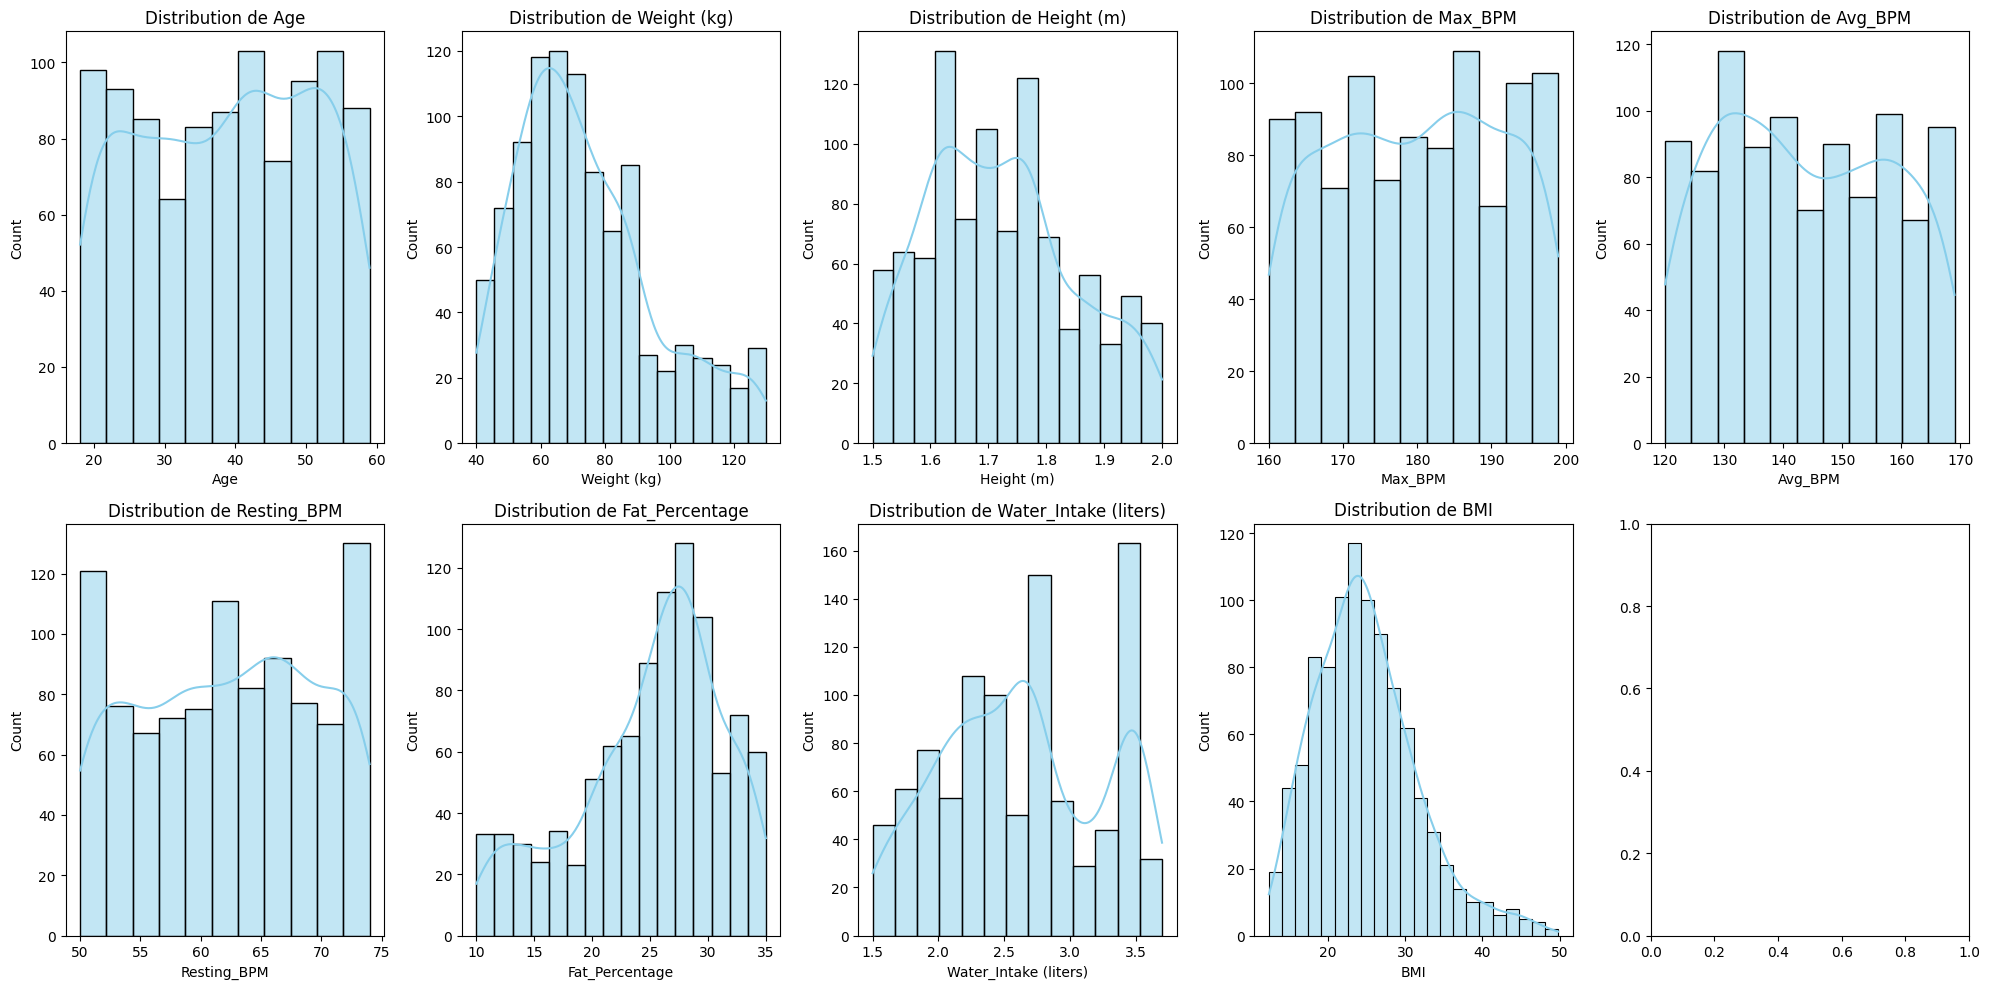
\includegraphics[width=0.7\linewidth]{distribution.png}
  \caption{Distribution des différentes variables}
\end{figure}

\begin{figure}[H]
  \centering
  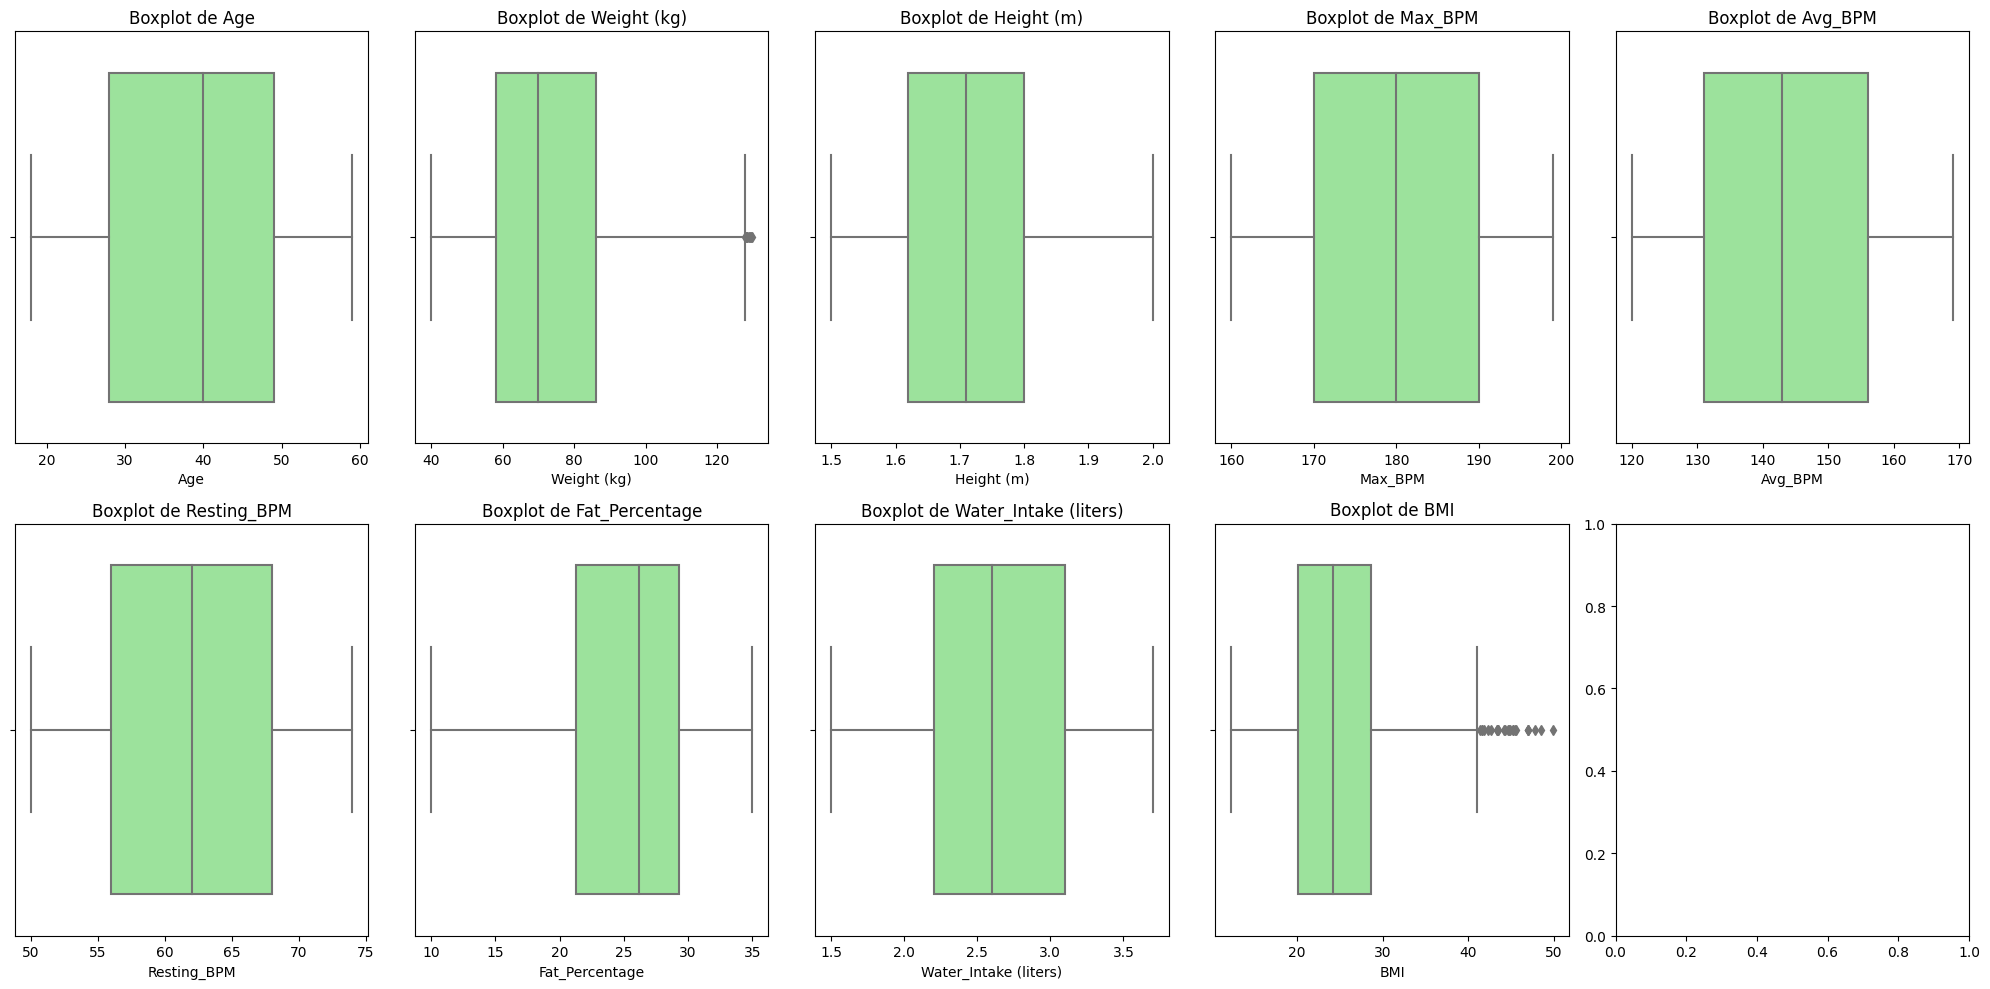
\includegraphics[width=0.7\linewidth]{boxplot.png}
  \caption{Boxplot des différentes variables}
\end{figure}

\subsection{Standardisation}
\textbf{But}:
Mettre les prédicteurs sur une même échelle (moyenne = 0, écart-type = 1) afin que les coefficients soient directement comparables en termes d’impact relatif.

\textbf{Exception}:
La variable cible, \texttt{Calories\_Burned}, reste en unité absolue pour que les métriques d’erreur (RMSE, MAE) gardent leur sens opérationnel (kcal).


\section{Exploration initiale}

\subsection{Distributions univariées}
Historiques et boxplots montrent que la plupart des variables (poids, IMC, calories) sont légèrement asymétriques, ce qui justifie la vigilance quant aux outliers.

\subsection{Corrélations}
La matrice de corrélation met en évidence :
\begin{itemize}
    \item Corrélation forte entre \texttt{Fat\_Percentage} et IMC (r = 0,75).
    \item Corrélation modérée entre \texttt{Avg\_BPM} et calories brûlées (r = 0,45).
    \item Faible corrélation de \texttt{Weight}, \texttt{Height} avec la cible une fois les autres variables prises en compte.
\end{itemize}

\begin{figure}[H]
  \centering
  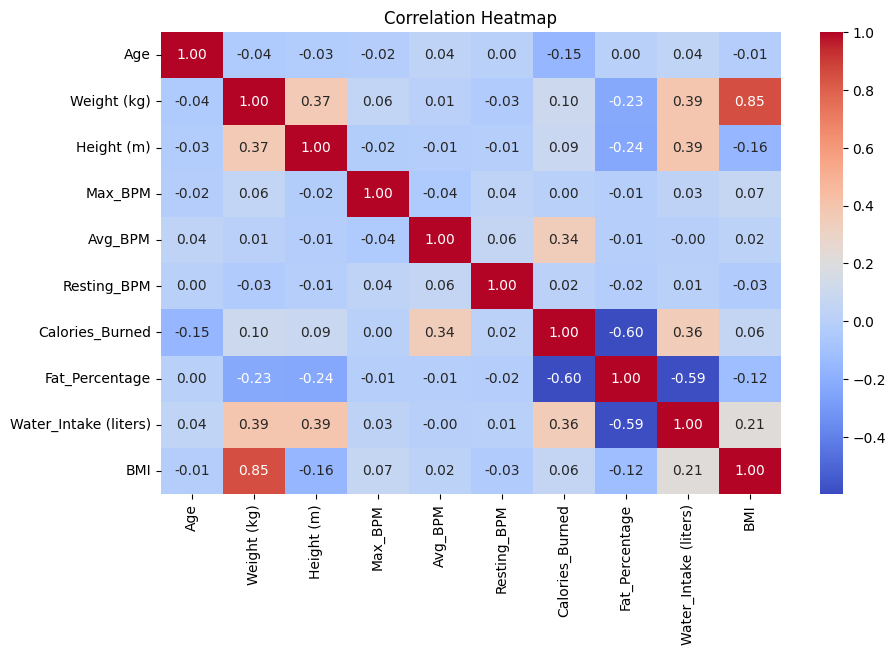
\includegraphics[width=0.7\linewidth]{correlation.png}
  \caption{Matrice de corrélation}
\end{figure}

\section{Modélisation initiale et diagnostic}

\subsection{Régression linéaire multiple complète}
\textbf{Résultats clés}:
\begin{itemize}
    \item R² = 0,50 (50\% de la variance expliquée).
    \item AIC/BIC élevés, F-statistic \begin{math}p < {10}^{-10}.\end{math}
    \item Variables significatives (\(p < 0,05\)) : \texttt{Age}, \texttt{Avg\_BPM}, \texttt{Fat\_Percentage}, \texttt{Water\_Intake}.
\end{itemize}

\subsection{Multicolinéarité}
\textbf{VIF}:
\begin{itemize}
    \item \texttt{Poids} : VIF = 70 ; \texttt{Taille} : VIF = 20 ; \texttt{BMI} : VIF = 64 → colinéarité extrême.
\end{itemize}

\textbf{Décision}:
Exclusion de \texttt{Weight} et \texttt{Height}, puis réévaluation.

\subsection{Modèle sans variables colinéaires}
Ajout des prédicteurs \{\texttt{Age}, \texttt{Avg\_BPM}, \texttt{Resting\_BPM}, \texttt{Fat\_Percentage}, \texttt{Water\_Intake}, \texttt{BMI}\}

\textbf{Résultats}:
\begin{itemize}
    \item VIF retombent tous < 2
    \item R² = 0,50, adj-R² = 0,49 → quasi-identique au modèle complet, diagnostic sensiblement plus stable.
\end{itemize}

\section{Sélection définitive : modèle réduit pas à pas}

\subsection{Critère de significativité}
Test F global de Fisher partiel pour regrouper les variables non-significatives (\texttt{Resting\_BPM}, \texttt{Water\_Intake}, \texttt{BMI}) : p > 0,1 → suppression simultanée légitime.

\subsection{Modèle final}
\textbf{Prédicteurs retenus}:
\begin{itemize}
    \item \texttt{Age} (coefficient négatif)
    \item \texttt{Avg\_BPM} (coefficient positif le plus élevé)
    \item \texttt{Fat\_Percentage} (coefficient négatif marqué)
\end{itemize}

\textbf{Performances}:
\begin{itemize}
    \item R² = 0,497 (49,7\%)
    \item AIC = 2101, BIC = 2120 (amélioration vs modèle complet)
    \item RMSE (standardisé) = 0,70 ; MAE = 0,52
\end{itemize}

\section{Diagnostics approfondis}

\begin{table}[H]
  \centering
  \caption{Résultats des tests de diagnostic}
  \begin{tabular}{ll}
  \toprule
  \textbf{Test / Graphique} & \textbf{Valeur / Observation} \\
  \midrule
  QQ-plot              & Alignement satisfaisant sur la diagonale (normalité quasi-respectée) \\
  Omnibus              & p = 0,00 (très sensible aux grands n ; compléter par JB) \\
  Jarque–Bera          & p = \(10^{-18}\) (léger excès de kurtosis, acceptable) \\
  Durbin–Watson        & = 2,10 (absence d’autocorrélation des résidus) \\
  Leverage (\(h_i\))   & Aucun point au-dessus de \(\tfrac{3(p+1)}{n}\) (p = 3) \\
  Cook’s D             & Toutes les distances < 0,5 → pas de points influents majeurs \\
  Rainbow test         & p = 0,08 (> 0,05) → linéarité globale validée \\
  \bottomrule
  \end{tabular}
\end{table}

\begin{figure}[H]
  \centering
  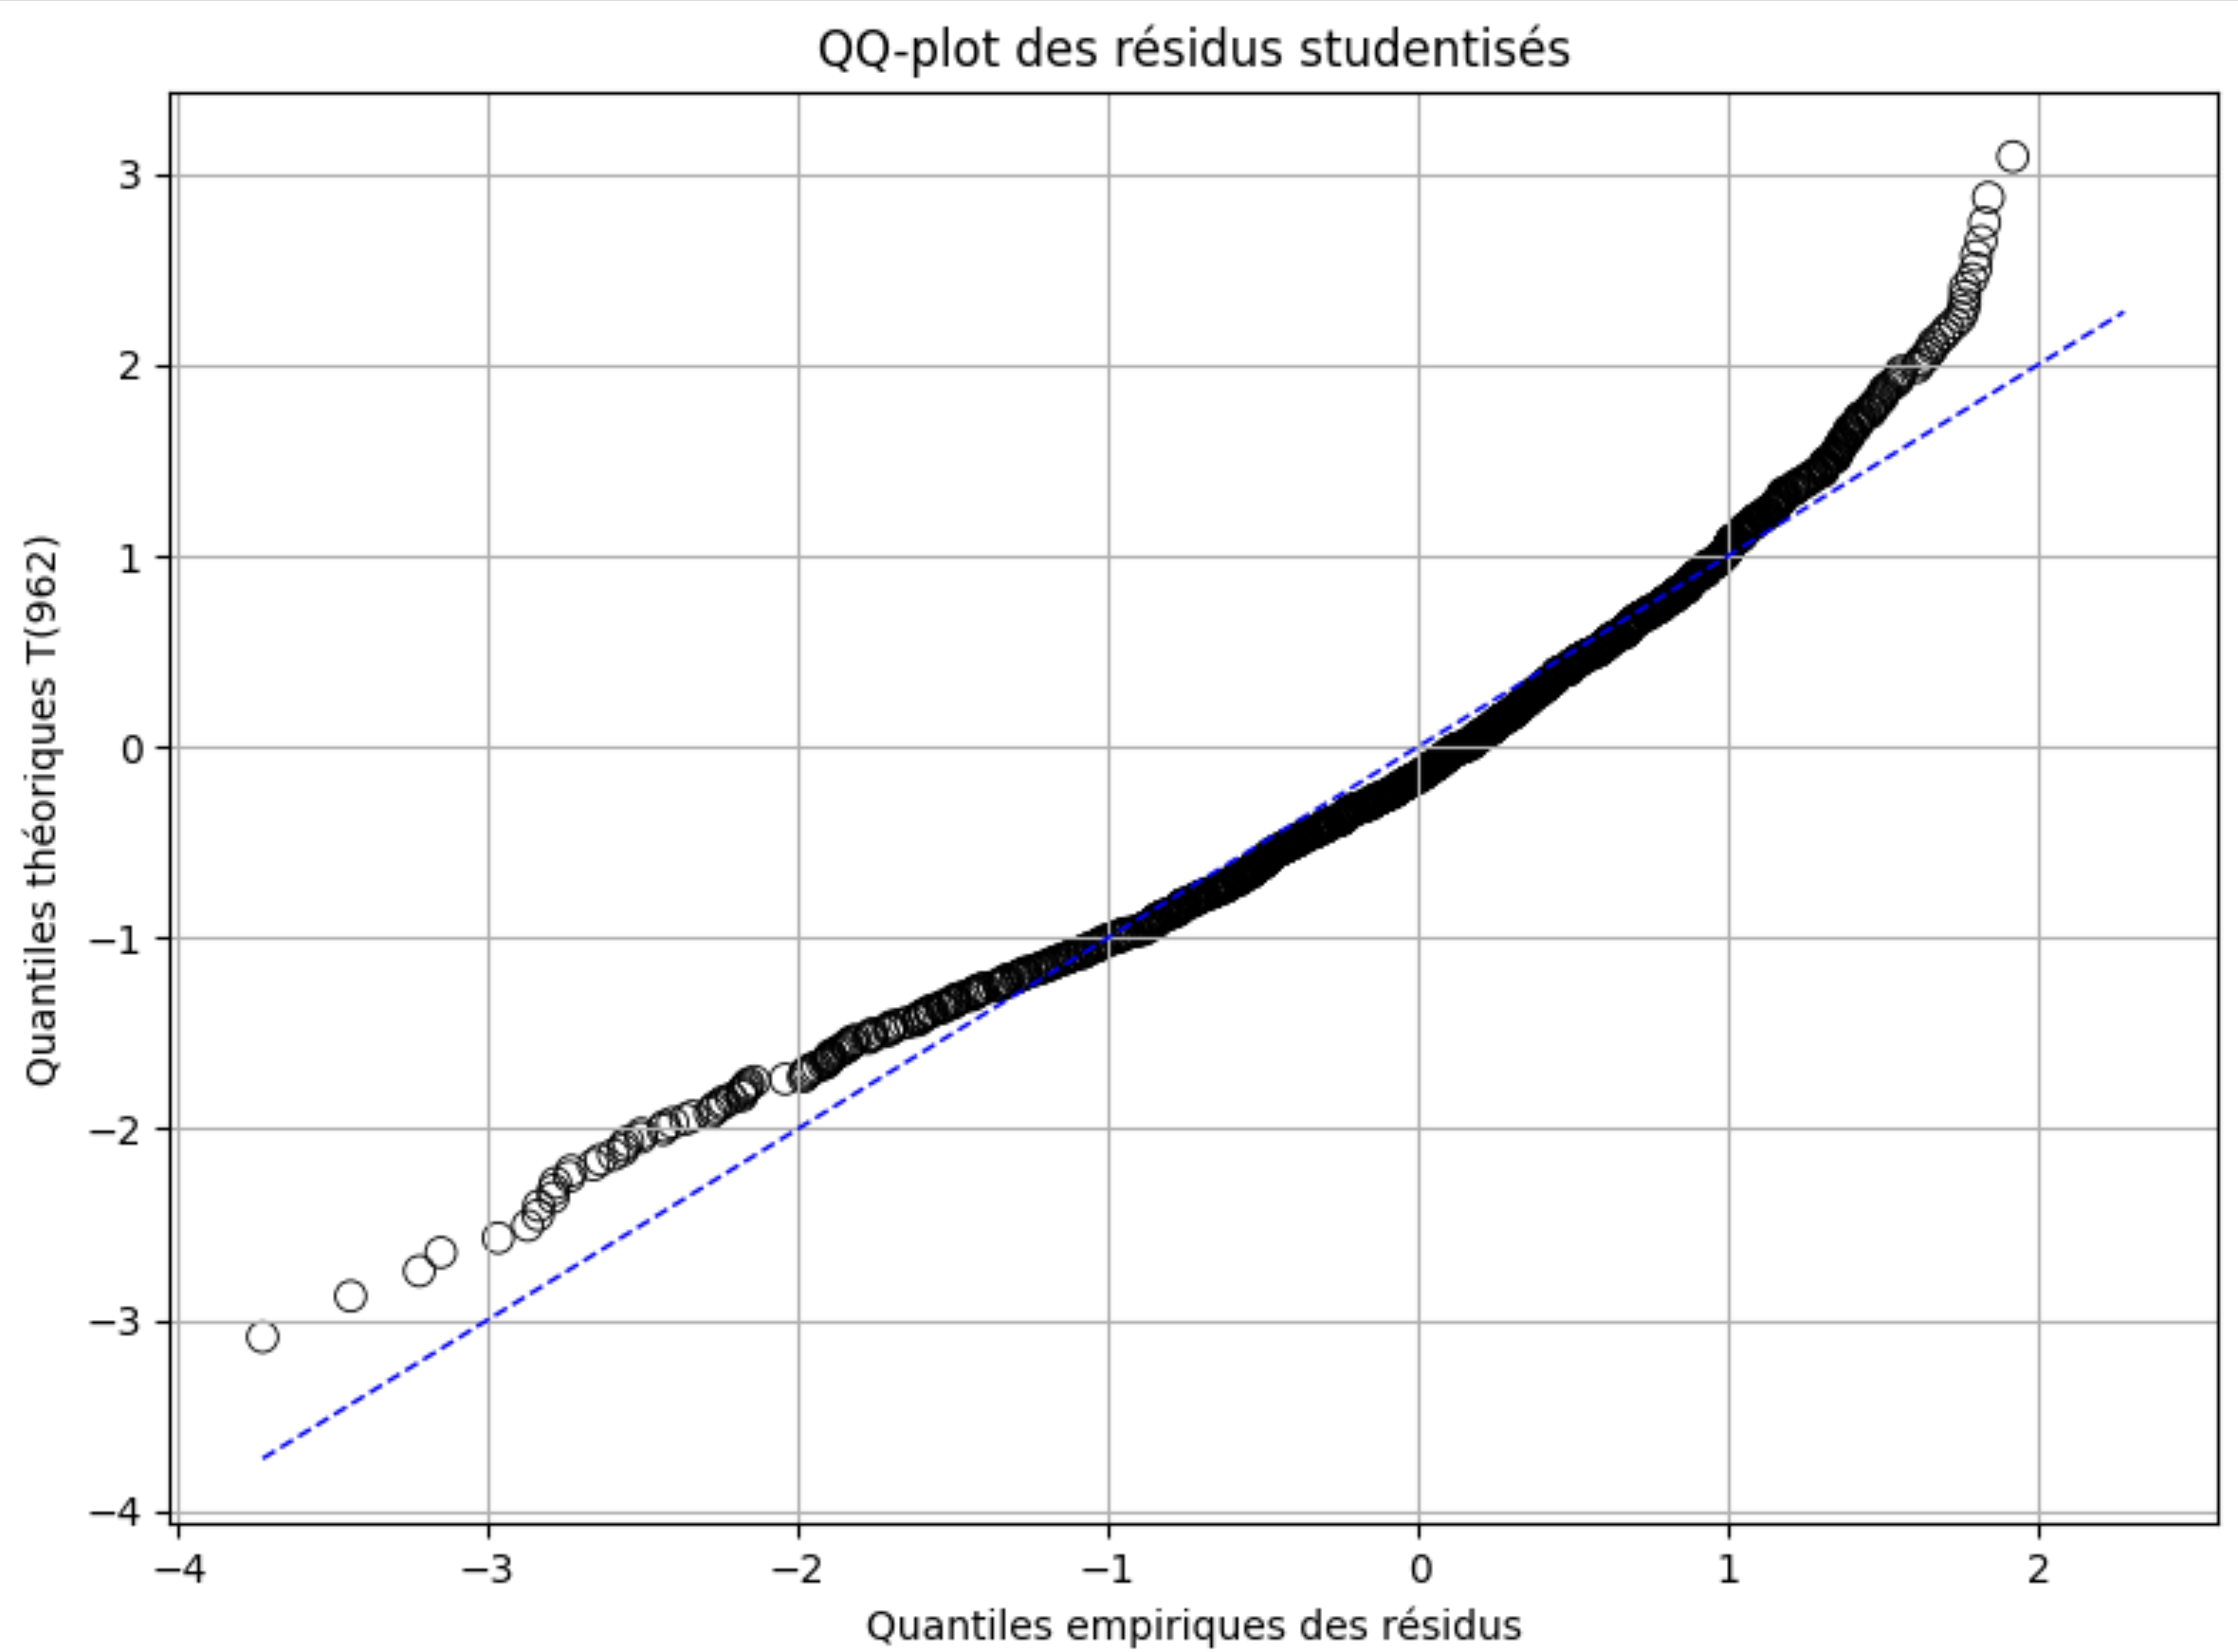
\includegraphics[width=0.7\linewidth]{qqplot.png}
  \caption{QQ-plot des résidus studentisés du modèle final}
\end{figure}

\section{Sélection de modèles supplémentaires}

\subsection{Vérification de la multicolinéarité (VIF)}
Après standardisation, les facteurs d'inflation de la variance (VIF) sont calculés pour chaque prédicteur :

\begin{table}[H]
\centering
\caption{VIF des variables explicatives}
\begin{tabular}{l r}
\toprule
Variable & VIF \\
\midrule
const & 1.00 \\
Age & 1.01 \\
Weight (kg) & 71.43 \\
Height (m) & 20.49 \\
Max\_BPM & 1.01 \\
Avg\_BPM & 1.01 \\
Resting\_BPM & 1.01 \\
Fat\_Percentage & 1.53 \\
Water\_Intake & 1.85 \\
BMI & 63.95 \\
\bottomrule
\end{tabular}
\end{table}

Sur la base de ces résultats, \texttt{Weight} et \texttt{Height} sont retirés pour stabiliser le modèle.

\subsection{Modèle sans variables colinéaires}
Le modèle réajusté inclut : Age, Avg\_BPM, Resting\_BPM, Fat\_Percentage, Water\_Intake, BMI.
\begin{itemize}
\item $R^2 = 0{,}498$, $R^2_{\text{ajusté}} = 0{,}495$
\item VIF < 2 pour toutes les variables.
\end{itemize}

\subsection{Modèle réduit par élimination pas-à-pas}
Une procédure de ``backward elimination'' retire simultanément Resting\_BPM, Water\_Intake et BMI (p > 0,10). Le modèle final retient :
\begin{itemize}
\item Age, Avg\_BPM, Fat\_Percentage
\end{itemize}
Avec :
\begin{itemize}
\item $R^2 = 0{,}497$, AIC = 2101, BIC = 2120
\item RMSE = 0{,}70, MAE = 0{,}52
\end{itemize}

\section{Recherche exhaustive et comparaison de modèles}
Une recherche exhaustive sur tous les sous-ensembles de variables permet de vérifier la robustesse de la sélection :
\begin{itemize}
\item 511 combinaisons évaluées par AIC, BIC, $R^2$, $R^2_{\text{ajusté}}$.
\item Le meilleur modèle à 3 variables (Age, Avg\_BPM, Fat\_Percentage) présente un AIC minimal ($\sim$2098) et un $R^2_{\text{ajusté}}$ optimal ($\sim$0,499).
\end{itemize}

\section{Validation croisée 5-fold et régularisation}

\subsection{Validation croisée}
Validation croisée 5-fold sur les modèles complet, sans colinéarité et réduit :
\begin{itemize}
\item Scores moyens de MSE, MAE, $R^2$ très proches entre complet et réduit.
\item Écart-type faible, confirmant la stabilité du modèle réduit.
\end{itemize}

\subsection{Ridge et Lasso}
Modèles pénalisés ajustés avec sélection de $\alpha$ par validation croisée interne :
\begin{itemize}
\item Ridge optimal : $\alpha \approx 1{,}0$, MSE moyen $\sim$0,48
\item Lasso optimal : $\alpha \approx 0{,}1$, MSE moyen $\sim$0,49
\item Conclusion : pas d’amélioration significative par rapport au modèle OLS réduit.
\end{itemize}

\section{Conclusion}
En conclusion, ce travail démontre que trois variables clés suffisent à expliquer près de 50 \% de la variabilité de la dépense calorique en séance de sport, facilitant l’interprétation et le déploiement du modèle. Les coefficients standardisés montrent que la fréquence cardiaque moyenne est le prédicteur le plus influent, suivi négativement par le pourcentage de masse grasse et l’âge. Ces conclusions offrent une base statistique solide pour adapter les programmes d’entraînement en fonction du profil physiologique des pratiquants. 

\newpage
\end{document}
